\documentclass[titlepage]{article}
\usepackage{school-style-packages}
\usepackage[cc]{titlepic}
\newcommand{\hi}[1]{\textbf{\textcolor{blue}{#1}}}

% For generating landscape orientated image, use Figure
\newenvironment{Figure}[1][!t]
  {\begin{landscape}\thispagestyle{empty}\begin{figure}}
  {\end{figure}\null\vfill\centerline{\raisebox{-2cm}{\thepage}}\end{landscape}}

\begin{document}
\title{Developer's Guide for PINSPEC}
\titlepic{
\includegraphics[width=\textwidth]{images/pinspec.png}}
\maketitle

\section{Introduction}
\subsection{Intro to Developer's Guide}
This document is meant to provide information in addition to the user guide hosted on \href{https://github.com/mit-crpg/PINSPEC/wiki}{GitHub's wiki pages}. A number of instructions on how to install the required packages and PINSPEC, how to set up the python input files, and how to run the code can be found on the above link. Some of these info may be repeated in this document, but as a general rule of thumb users should refer to the wiki page for instructions related to using PINSPEC, and this document is reserved for info on developing PINSPEC. 

While the rest of this section would provide a high-level introduction of how PINSPEC source codes are constructed, the next couple of sections in this document would be devoted to:
\begin{itemize}
\item Review some essential instructions for installing PINSPEC and running PINSPEC, see Section~\ref{install}. 
\item Discuss how to manipulate the python codes, see Section~\ref{python}.
\item Discuss how to manipulate the C++ codes, see Section~\ref{C++}. 
\end{itemize}
Keep in mind that the above info is in addition to the commenting in the source codes and Doxygen-generated files as hosted here: \href{http://mit-crpg.github.io/PINSPEC/index.html}{Doxygen generated documents}. 


\clearpage
\subsection{Python to SWIG to C++}
Fig.~\ref{high-level} illustrates the three major components of PINSPEC: the python codes, the SWIG interface, and the C++ source codes. 

Simplified Wrapper and Interface Generator (SWIG) is open source software used in PINSPEC to wrap C++ functions for use with python. More generally, SWIG can be used to connect C/C++ with scripting languages such as Lua, Perl, PHP, Python, R, Ruby, Tcl and even non-scripting languages like C\#, Java, JavaScript, Go, Modula-3, Ocaml, Octave, and Scheme\footnote{Reference: \href{http://en.wikipedia.org/wiki/SWIG}{SWIG's wiki page}, \href{http://www.swig.org/exec.html}{SWIG's homepage}.}. 

More specifically, here is the flow of a typical simulation:
\begin{itemize}
\item Users inputs data in a python file;
\item PINSPEC python source codes process input data, perform Doppler Broadening of the cross sections if requested;
\item SWIG registers the data in C++ classes;
\item C++ contains the actualy Monte Carlo kernel, and neutrons are simulated here;
\item If any plotting is requested, generated results would be passed from C++ back to python using SWIG again and python would generate plots. 
\end{itemize}
\begin{figure}[h]
  \centering
  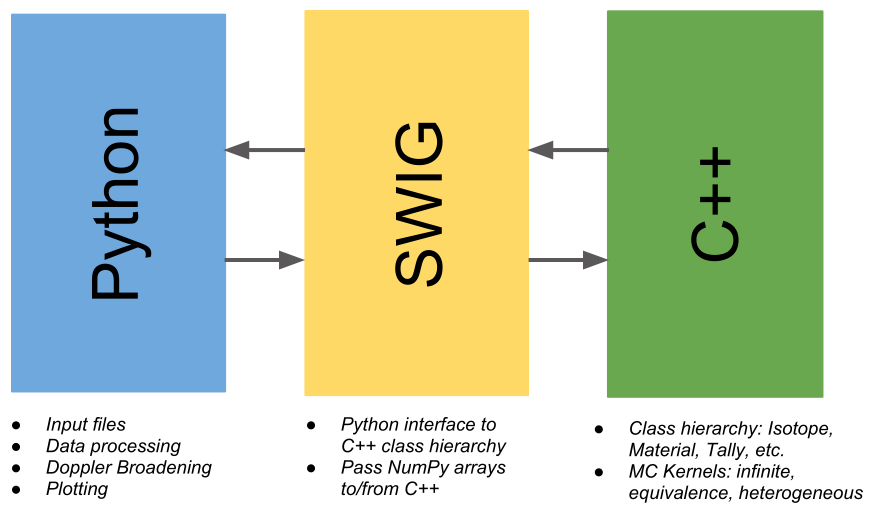
\includegraphics[width=5in]{images/high-level.png}
  \caption{Python Interfacing C++ Through SWIG} \label{high-level}
\end{figure}


\clearpage
\subsection{Major C++ Classes and Structures}
C++ using the following major classes and structures: 
\begin{enumerate}
\item Geometry: the umbrella object that knows the \# neutrons per batch, \# batches, \# threads, the type of geometry etc. Geometry contains region, which contains material, which contains isotopes. There are three types of geometries:
  \begin{itemize}
  \item \hi{Infinite homogeneous model}: that is, the entire geometry is one homogenized material. 
  \item \hi{Heterogeneous equivalent model}: that is, the region declared as Equivalent Fuel would be homogenized into one fuel region, and the region declared as Equivalent Moderator would be homogenized into one moderator region, and we use collision probability method to estimate the probability of neutrons traveling from one region to another. In this model neutrons only know whether they are in Equivalent Fuel or Equivalent Moderator and do not have an explicit $(x,y,z)$. 
  \item \hi{Full heterogeneous model}: this is the model where neutrons truly know their $(x,y,z)$ locations. In this model, region objects contain surfaces.
  \end{itemize}
  
\item Region: a region object knows its region name, the material inside, its region type, volume and buckling. More specifically, we support 6 region types: 
  \begin{itemize}
    \item \hi{Infinite medium}: this region covers an infinite space. 
    \item \hi{Equivalent fuel}: this region is a fuel region using the infinite equivalence model. 
    \item \hi{Equivalent moderator}: this region is a moderator region using the infinite equivalence model. 
    \item \hi{Bounded fuel}: this region is a fuel region using the true heterogeneous model. 
    \item \hi{Bounded moderator}: this region is a moderator region using the true heterogeneous model. 
    \item \hi{Bounded general}: this region is a generalized region bounded by surfaces and is used in the true heterogeneous model. 
  \end{itemize}
  %See Fig.~\ref{classRegion} for an illustration of the inheritance structure of the Region class. 
  \begin{figure}[h]
    \hspace{-1in}
    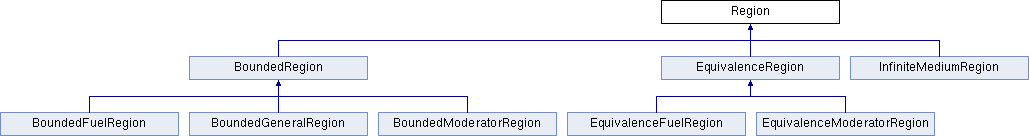
\includegraphics[width=1.5\textwidth]{images/classRegion.png}
    \caption{Inheritance Diagram of Region Class} \label{classRegion}
  \end{figure}



\item Surface: Surface objects are used to bound regions in the true heterogeneous model. A surface object knows its name, ID \#, its surface type (three sub-classes: x-plane, y-plane, z-cylinder), and its boundary condition (reflective, vacuum, interface). 
  \begin{figure}[h]
    \centering
    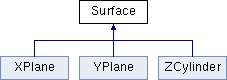
\includegraphics[width=0.5\textwidth]{images/classSurface.png}
    \caption{Inheritance Diagram of Surface Class}
  \end{figure}


\item Material: an material object contains one or more isotope objects, and an material object is used to filled a region object. A material object knows basic info like its name, ID \#, material density; when adding an isotope into a material, the material object needs to know the relative atomic mass associated with each isotope. 
  \begin{itemize}
  \item Note: each material and isotope isotope object needs to keep track of its number densities. Instead of having users to manually put in number densities, PINSPEC keeps track of them; notice that every time a new isotope is added, the number density of the material as well as other isotopes need to be updated as well. PINSPEC handles it by keeping a map of the isotopes with its corresponding relative atomic mass in each material object. So every time a new isotope is added, the material object loops through all existing isotopes and update the number density of the material and of each isotope. 
  \end{itemize}

\item Isotope: an isotope object can be considered as one of the most basic object in PINSPEC. We use isotope to build material, which in turn builds region, which builds geometry. An isotope object needs to have a name and atomic number, and PINSPEC would assign each isotope a unique identifier, calculate its $\displaystyle \alpha = \left(\frac{A-1}{A+1}\right)^2$, $\eta, \rho$ for SLBW, averaged cosine of scattering angle $\displaystyle \bar{\mu} = \frac{2}{3A}$ etc. 
  \begin{itemize}
    \item We asks the user to provide isotope name in the format of: isotope's periodic table name (first letter capitalized), followed by its atomic number, with a hyphen in-between.
  \end{itemize}

\item Neutron: a neutron structure knows its batch number (for running multiple batches and performing batch statistics), its previous energy (in eV) and its current energy (in eV), the region it is in, the material it is in, and the isotope it is in. For heterogeneous geometries, neutrons also know its $(x,y,z)$ location, $(u,v,w)$ velocity directions, and the closest surface. This neutron structure is being passed from class to class, and it contains the most essentially information that the other classes would depend on to perform the simulation and generate the corresponding statistics. 

\item Tally: PINSPEC uses a Tally class to keep the implementation of tally accumulation general. See Fig.~\ref{classTally} for the different sub-classes supported in the Tally class. There are also a TallyBank class that stores all the tallies, and a TallyFactory class that creates tallies. For more details, see Section~\ref{example-add-tally} for an example on how to implement a new tally type. 
  \begin{Figure}
    \vspace{-1in}
    \hspace{-1.45in}
    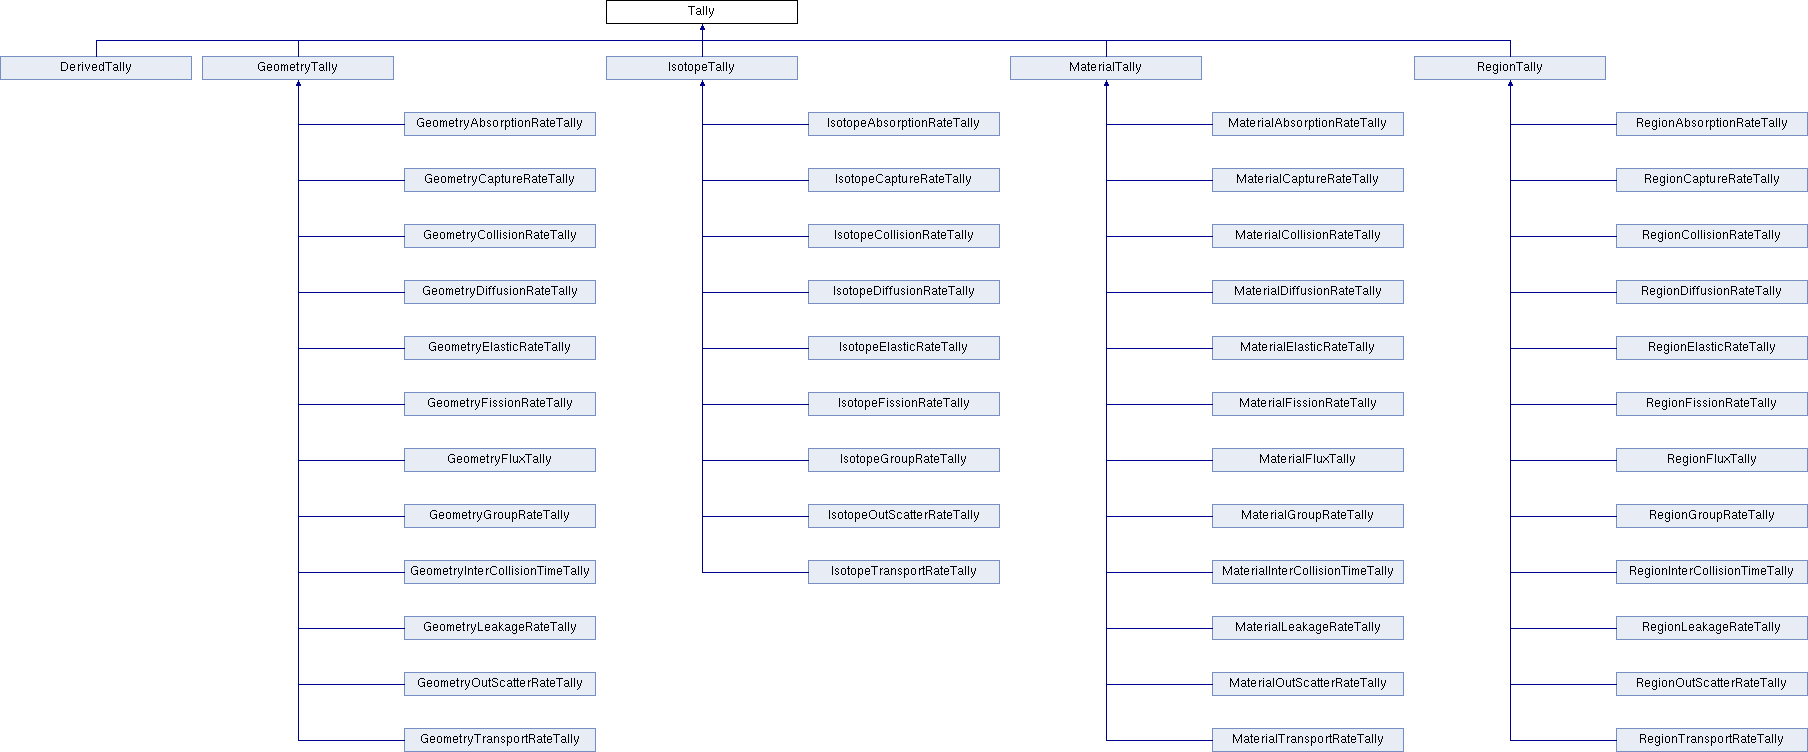
\includegraphics[width=2.\textwidth]{images/classTally.png}
    \caption{Inheritance Diagram of Tally Class} \label{classTally}
  \end{Figure}
\end{enumerate}




%%%%%%%%%%%%%%%%%%%%%%%%%%%%%%% INSTALL %%%%%%%%%%%%%%%%%%%%%%%%%%%%%%%%%
\clearpage
\section{Installation and How To Run} \label{install}
An overview of the installation procedures can be found on the users' guide at \href{https://github.com/mit-crpg/PINSPEC/wiki/Installing-PINSPEC}{PINSPEC's wiki page}. 

Table.~\ref{install-table} lists PINSPEC's package requirements and the third column provides installation suggestion for ubuntu users. 
\begin{table}[h]
  \centering
  \begin{tabular}{|c|c|c|} \hline
    Package & Version \# & Installation \\ \hline \hline
    Python & 2.7 & sudo apt-get install python2.7 \\ \hline
    matplotlib & 1.2 or later & sudo apt-get install python-matplotlib \\ \hline
    numpy & 1.6 or later & sudo apt-get install python-numpy \\ \hline
    scipy & 0.9 or later & sudo apt-get install python-scipy \\ \hline
    SWIG & -- &  sudo apt-get install swig \\ \hline
    GIT & -- & sudo apt-get install git \\ \hline
  \end{tabular} 
  \caption{PINSPEC Package Requirements and Installation Notes} \label{install-table}
\end{table}
Notes:
\begin{itemize}
\item Ubuntu users: 
\begin{itemize}
\item If you have Ubuntu v12.10, the default installation (aka using the commands listed in Table~\ref{install-table}) would get you the right versions. 
\item If you have an earlier version of Ubuntu, and the packages you obtained through your Ubuntu release are earlier versions than the ones listed in Table.~\ref{install-table}, we suggest you first install all the packages required, and try running PINSPEC, and python's error message would help you determine whether you need any newer version of software. 
\item If you tried the previous bullet point and decided you have to build some of these packages from source, here are examples for pulling numpy and scipy from their git repositories: 
\begin{verbatim}
> git clone git://github.com/numpy/numpy.git numpy 
> git clone git://github.com/scipy/scipy.git scipy
\end{verbatim}
Then build using python's utilities:
\begin{verbatim}
> python setup.py install
\end{verbatim}
For more details, see \href{http://scipy.org/Installing_SciPy/BuildingGeneral}{Scipy's installation page} for instance. 
\end{itemize}

\item Other Linux users: use your corresponding package management system. For instance, in Gentoo you would use `emerge' to get the above packages. 

\item Mac users: try install the listed packages using MacPort, and MacPort seems to be the Mac version of package management system, and it should make keeping track of dependencies and updating packages in the future easier. 
\end{itemize}


\clearpage
\subsection{A Special Note About Python Version and Running Python}
\begin{itemize}
\item Python2 vs. Python3: because of the syntax incompatibility between python2 and python3, PINSPEC only supports python2 (more specifically it is tested mostly with python2.7). Developers could choose to update the python source codes into python3 syntax in the future if python3 gets more popular; though for now the easiest thing to do for users with python3 would be to install a copy of python2.7 as well, and every command that has `python' in it, using the syntax `python2.7' would request the correct version of python. 

\item We provide a setup.py file in the release that would build PINSPEC using \href{http://docs.python.org/2/distutils/index.html}{distutils}. To run in Linux:\begin{verbatim}
> python setup.py install --user
\end{verbatim}
The `--user' flag is handy for two reasons: a) you do not need root access later to run etc; b) you do not want to build PINSPEC into the default directories on your machine that keep your real programs.

\item Mac users may run into problems with running our python setup.py file (located in the main directory). It is recommended to use the env prefix as in the following example for users with gcc-4.7:
\begin{verbatim}
> env CC=gcc-mp-4.7 python setup.py install --user
\end{verbatim}
\end{itemize}

\clearpage
\subsection{Additional Tools}
This section contains some notes on useful tools that developers might find beneficial. Notice this is by all means an incomplete list and would be updated from time to time. 
\begin{enumerate}
\item Version control/source code management. We choose to use GIT (and use gitHub as our host for repositories), so it is recommended that the developers use git as well. However if you really insist, there might be a way to set up such that you can continue to use SVN, which is supported by GIT now, though we would be at the risk of losing our commit log messages. 


\item Secure Copy (SCP) is useful in securely transferring files between two hosts. Two hosts can be: your local machine, and the server that you might run PINSPEC on. More specifically, the general command for copying a file from a local folder to a remote folder is: 
\begin{verbatim}
> scp <local folder path> <account>@<ip>:<remote folder path>
\end{verbatim}
For coying files from a remote folder to a local machine, you just need to need to swap the second and third argument. 

\item SSHFS enables mounting of a remote filesystem on a local machine. That is,  you can mount a remote directory (say, the one you have on a server) onto your laptop, and you can access it graphically using your file management system (e.g., click open a file, edit it, etc). Here are the three common commands:
\begin{itemize}
\item To mount: 
\begin{verbatim}
> sshfs -0 idmap=user <account>@<ip>:<remote folder path> <local folder path>
\end{verbatim}

\item To see what sftp subsystems are mounted: 
\begin{verbatim}
> ps aux | grep -i sftp | grep -v grep
\end{verbatim}

\item To unmount: 
\begin{verbatim}
> fusermount -u <local folder path>
\end{verbatim}
\end{itemize}

\item To be continued. 
\end{enumerate}






%%%%%%%%%%%%%%%%%%%%%%%%%%%%%%% PYTHON %%%%%%%%%%%%%%%%%%%%%%%%%%%%%%%%%
\clearpage
\section{Manipulating Python Inputs}\label{python}
\subsection{Utilizing Tally Arithmetic}
In writing the python input file, users can utilize the tally arithmetics implemented and create essentially a new tally type by `adding,' `subtracting,' `multiplying,' and `dividing' two existing tallies together. 

There are three tally arithmetics supported in PINSPEC using operator overload; we use addition as an example:
\begin{enumerate}
\item `new\_ tally = tally1 + tally2': after error checking (e.g., tallies have computed batch statistics, tally1 and tally2 have the same \# of energy bins), a new tally (of derived type) of the correct length will be initialized, and entry $i$ in new\_tally would be the addition of tally1[$i$] $+$ tally2[$i$]. 
 
\item `new\_tally = tally1 + 3.5': a new tally (of derived type) will be initialized to have the same length as tally1, and for every entry $i$, new\_tally[$i$] = tally1[$i$] + 3.5. Notice PINSPEC only supports tally $+$ constant, not constant $+$ tally. 

\item `new\_tally = tally1.addFloats(numpy.array([1,2]))': instead of the second argument being a single number, users can choose to pass in an array of numbers as well using numpy. In addition to addFloats(..), PINSPEC also supports addIntegers(..), or addDoubles(..). 
\end{enumerate}
For more details, see Tally.cpp's operator overloading functions. 

If the tally you want cannot be implemented this way, see Section.~\ref{example-add-tally} for suggestions on how to implement your own tally types. 


\clearpage
\subsection{Example: Add A New Isotope}
The PINSPEC package comes with a library of common isotopes' ENDF/B-VII cross sections for capture, elastic scattering and fission cross sections. 
\begin{itemize}
\item To view the isotopes available, developers can do a `ls' in PINSPEC/pinspec/xs-lib. 
\item To add a provided isotope to your simulation, call Isotope construct with the isotope name (formatted as the isotope's periodic table element name followed by hyphen followed by atomic mass). For instance, 
\begin{verbatim}
U235 = Isotope('U-235')
O16 = Isotope('O-16')
Zr90 = Isotope('Zr-90')
\end{verbatim}
\end{itemize}
If an isotope of desire is not included in the xs folder, following the instruction in the next sub-section on how to define your own isotope cross section, and construct isotope object the same way as if the isotope is a PINSPEC pre-defined one.


\clearpage
\subsection{Example: Add A New Cross Section}
It is also possible to add to this library and use other isotopes from the ENDF/B-VII cross section library. To do this, visit the National Nuclear Data Center and follow the steps below:
\begin{itemize}
\item Select the element you wish to add to the library.
\item On the right hand side, select the isotope.
\item On the right hand side, select the `plot' link next to the cross section desired ((n,elastic), (n,gamma) or (n,total fission)). A new tab will appear.
\item On the right hand side, click "view evaluated data".
\item At the top of the page, scroll over the link called "Text". Right click and select `Save Link As..'. This will give you the option of saving the cross section file as a text file.

\item Save the above file in the xs-lib folder (PINSPEC/pinspec/xs-lib), and title it with the element abbreviation, mass number, and isotope designation. For example, the capture cross section (n,gamma) for Boron 10 should be saved as B-10-capture.txt. 

\item Then you can use it as any pre-defined isotope types. 
\end{itemize}





%%%%%%%%%%%%%%%%%%%%%%%%%%%%%%% C++ %%%%%%%%%%%%%%%%%%%%%%%%%%%%%%%%%
\clearpage
\section{Manipulating C++ Codes}\label{C++}
\subsection{Create A New Source File}
If you create a new source file, make sure do the following: 
\begin{enumerate}
\item Add it to \textit{setup.py}

\item If you need to pass data from the python input file into the C file, or you would like to retrieve the results generated by C++ and plot or print it using python, see Section~\ref{data}. 

\item Make sure you update the doxygen commenting accordingly, and run doxygen by:
\begin{verbatim}
 doxygen docs/Doxyfile
\end{verbatim}
See more details in Section.~\ref{doxygen}. 

\item If you add in any additional functions, it is nice to update the test suites accordingly. 

\item Two examples are shown about how to add a new tally and a new surface. 
\end{enumerate}



\clearpage
\subsection{Passing Data Between Python and C++} \label{data}
If you would like to gain access to an array of data, you need to do so through SWIG. Currently we have Geometry.i to keep track of the data being passed between the two programs, and to add your own, for instance, you need to do something similar to the following: 
\begin{verbatim}
%apply (float* ARGOUT_ARRAY1, int DIM1) {(float* xs, int num_xs)}
\end{verbatim}
The above means that a (float *xs, int num\_xs) argument in C++ can be translated into an array ARGOUT\_ARRAY1 of length DIM1. 


Examples can be found in Geometry.i which contains numpy template. 



\clearpage
\subsection{Doxygen Commenting} \label{doxygen}
To generate html and pdf from source code commenting, run Doxygen by the following command:
\begin{verbatim}
 doxygen docs/doxygen/Doxyfile
\end{verbatim}

If you modify the source code, please update the Doxygen commenting accordingly. For instance, here are some styling suggestions:
\begin{enumerate}
\item For any class structure (including super-class and sub-class), use @class followed by class name, header file name, and header file path. Examples:
\begin{verbatim}
@class Surface Surface.h "pinspec/src/Surface.h"
@class XPlane Surface.h "pinspec/src/Surface.h"
@class YPlane Surface.h "pinspec/src/Surface.h"
\end{verbatim}
In the above examples, Surface is the super-class, and XPlane and YPlane are sub-classes. 

\item For any structure, try using @brief followed by a one-line short description, as well as @details followed by a longer description if needed. 

\item For any structure, use @param followed by parameter name and description to comment on the inputs of a method, and use @return followed by variable name and description to comment on the outputs of a method. 
\end{enumerate}


\clearpage
\subsection{Update Test Suites}

\clearpage
\subsection{Example: Implement A New Surface}

\clearpage
\subsection{Example: Implement A New Tally} \label{example-add-tally}


\clearpage
\subsection{Example: Implement A Monte Carlo Variance Reduction Technique}
The main kernel that performs the Monte Carlo simulation is contained in Geometry.cpp as runMonteCarloSimulation(). 

\begin{algorithm}

\caption{High Level Monte Carlo Kernel}
\begin{algorithmic}
\FOR{each batch}
\FOR{each neutron inside the batch}
\STATE Initialize neutrons:

\ENDFOR
\ENDFOR
\end{algorithmic}
\end{algorithm}

\end{document}
